%1 

\chapter{Introduction}
%%\hypertarget{RefHeading18281935131865}


\section{Background}
%%\hypertarget{RefHeading18301935131865}

''Mauwake used to be a big language. The neighbours knew it too, and it was used as a trade language in the area. But today it is not so important any more.'' This is what my colleague Kwan Poh San and I heard when we settled among the Mauwake people in the late 1970's to do linguistic and Bible translation work. Especially before the second World War everybody, including the Mauwake speakers themselves, knew their neighbours' languages better than nowadays, but it may also be true that Mauwake did have a stronger position among the languages in the area. And it is certainly true that the language is fast losing ground to Tok Pisin (also called Melanesian Pidgin), the trade language \textit{par excellence} in Papua New Guinea today.  The process is so strong that Mauwake can be considered an endangered language.

\section{Purpose and theoretical orientation of the study}
%\hypertarget{RefHeading18321935131865}
\subsection{Purpose}
%\hypertarget{RefHeading18341935131865}
My aim is to give a synchronic description of grammatical structures and their functions in Mauwake. Occasionally some attention is given to diachronic aspects as well, when that is considered interesting or helpful for understanding the system at present \citep[20]{EvansEtAl2006}%Dench
. 

This grammar covers mainly morphology and syntax, but a brief overview of phonology is also given, and some pragmatic features are discussed very briefly at the end. A short introduction to typological features and the basic clause structure is given in the introduction to familiarise especially those readers a little with the language who are not reading the grammar from the beginning to the end. The description proper of  the morphology and clausal syntax starts from the structures and describes their functions, as the basic structural features need to be understood first to get a good idea of the language \citep[59]{Mosel2006}. But since functional domains increase in importance when one moves higher up in the unit hierarchy, this is reflected in the arrangement of the grammar: the syntax above the clause level starts from functions and describes different structures used for those functions. Another reason for this switch from an analytic (form-based) to a synthetic (function-based)\footnote{The analytic approach is also called \textit{onomasiological} and synthetic approach \textit{semasiological}.}  approach is the desire to make the grammar more useful for typologists (\citealt{Cristofaro2006} and \citealt[15]{EvansEtAl2006}). 

The size of the grammar presents a challenge as to the relative amount of documentation vs. analysis.  While documentation is the main purpose of this work, I have attempted to present enough of the analysis to show the reader reasons for certain choices,\footnote{E.g. the status of adjectives as a separate word class and the question of serial verbs have received more discussion than some other topics.} even if I may not meet \citegen[132]{Dixon1997} requirement of justifying all my choices ``with a full train of argumentation''.


This grammar does not include a vocabulary, as a Mauwake dictionary \citep{JarvinenEtAl2001} is available electronically.



\subsection{Theoretical considerations}
%\hypertarget{RefHeading18361935131865}
In the analysis and writing I have been following the informal descriptive theory that was only recently given the name Basic Linguistic Theory (\textsc{blt}) by \citet{Dixon1997} and elaborated by him (\citeyear{Dryer2010}--\citeyear{Dryer2012}) and by \citet{Dryer2006a, 2006b}, who also defends its status as a legitimate linguistic theory. \textsc{blt} makes use of the cumulative knowledge acquired during decades, and centuries -- even millennia -- of grammatical studies, and in the writing of descriptive grammars \citep[3]{Dixon2010}. It is largely based on traditional grammar, but in contrast to traditional grammar it aims to describe the `essential nature' of each language rather than fitting the language into a pre-determined formal model\footnote{These models are often called ``theories''.  For a comment on this, see \citet[131]{Dixon1997}. \citet{Dryer2006a} prefers to call them theoretical frameworks.} \citep[211]{Dryer2006a}. Each language is seen ``as a complete linguistic system'' on its own \citep[4]{Dixon2010}. The theory has been modified over time, and is continually being modified, by developments in typological and formal linguistics (\citealt{EvansEtAl2006}, \citealt{Rice2006a, Rice2006b}, \citealt[3]{Dixon2010}).  

Even if \textsc{blt} does not try to fit languages into any predetermined formal model, it may borrow formalisms from various models as far as they are appropriate and helpful for the description of a particular language \citep[128--135]{Dixon1997}.\footnote{Among others promoting the use of \textsc{blt}, whether they use the name or not, are
\citet[354]{Noonan2006}, 
\citet{Rice2006a, Rice2006b}, 
\citet{EvansEtAl2006}, and \citet{Payne1997, Payne2006}.}  \textsc{blt} is closely linked with language typology, ``[setting] out a typological paradigm, by inductive generalization from reliable grammars'' \citep[205]{Dixon2010}. \citet[6]{EvansEtAl2006} note that grammars written in this framework tend to stand the test of time better than those following strict formal models. Formal theories have been and are useful in providing useful research questions -- both bringing up completely new ones and deepening old ones -- and in forcing the descriptions to be more rigorous. In \citegen[262]{Rice2006b} words, ``[t]he theory informs and shapes, but does not control''. 




My own dislike of formalisms is certainly one reason why they are used so little in this grammar.  A more important factor is my desire to make the grammar readable to as many people as possible regardless of their linguistic background. This is also reflected in the use of terminology. I have tried to use widely accepted and transparent terminology as much as possible, to avoid technical terms specific to some particular formalism, and to explain my terminology where necessary (cf. \citealt{Cristofaro2006}). 

For the description of Mauwake the following basic concepts familiar from traditional grammar are assumed as given:

Word classes like noun, verb, pronoun, adverb (the status of adjective as a class of its own is discussed separately);

Morphological cases like nominative, accusative, genitive and dative;

Syntactic roles of subject and object;

Semantic/case roles like agent, patient, recipient and beneficiary;

Phrases like \textsc{np}, \textsc{ap}, \textsc{AdvP};

Clause as a separate level from sentence. 

The concept of medial verbs, as against final/finite verbs, which is generally accepted in Papuan linguistics, is also presupposed. 

Since frequency of occurrence is an important and interesting characteristic of grammatical usage, I initially planned to do a fair amount of quantification and frequency counting.  But to do an adequate job would have required a much larger corpus, as well as better computer programs and knowledge of corpus linguistics, and much more time, than I had at my disposal. Even though actual percentages are seldom mentioned in the final product, I have occasionally included frequency statements based on whatever frequency counts I have made during the course of the work and on my personal experience with Mauwake. 

To my knowledge there are no trained linguists among the Mauwake speakers, so the kind of cooperation between a native and a non-native speaker linguist, together with native speaker non-linguists, that \citet{Ameka2006} advocates, was not possible.  Even though I have aimed at checking the material as carefully as possible, there are bound to be mistakes both in the data and in the interpretation. It is necessary to heed Ameka's (ibid. 92) warning that ``[o]ne of the most dangerous things about authoritative and influential foundation records ... is that their misanalyses which pertain to some theoretical or typological point are repeated over and over again in the literature.  What is even worse is that the theories and generalizations are built on such mistakes''. 

\subsection{Audience} 
%\hypertarget{RefHeading18381935131865}
One can anticipate the readership for a reference grammar of a previously undocumented and endangered language spoken by a couple of thousand speakers to consist mainly of linguists.  I especially hope this grammar to be useful for those linguists who work on language typologies and typology-related questions. Naturally the material is also available for those interested in more formal models.

A grammar is expected to describe features that exist in a language, rather than those that do not exist. But for the benefit of typologists I have at times mentioned the non-existence of certain features that they might be looking for and wondering about, if there is no mention at all \citep{Cristofaro2006}. 

Another readership I want to address are those people particularly in Papua New Guinea who are linguistically somewhat less trained, yet are vitally interested in language development and translation.  If this grammar helps any of them to study and understand a language better, or encourages someone to write a grammar of yet another undocumented language, my work has been worthwhile.

It is unlikely that many outsiders would use this grammar to learn Mauwake.  It may also be unrealistic to wish that many Mauwake speakers would become familiar with it. Yet it is my desire that it would help the Mauwake speakers in at least two ways: by preserving their language and giving them more pride in it as they realise that it does have a real grammar \citep[255]{Kadanya2006}, and also by providing some help for those interested and involved in teaching vernacular literacy.

\subsection{On the data and examples} 
%\hypertarget{RefHeading18401935131865}
The bulk of the text data used for this grammar were collected between 1979 and 1985, with some later additions. The basic data of 19 spoken and 7 written texts contain over 8300 words in all (200+ \textsc{kb} in plain text), edited by a native speaker. They consist mainly of narratives, also including traditional stories (60\%), but descriptive texts (15\%), process descriptions (14\%) and one long hortatory text (11\%) are included as well, from different speakers and authors.\footnote{Appendix 1 provides a list of the texts used.} Many syntactic features were further checked against another set of texts about the same size. 

When choosing examples, I have taken as many from text material as possible, especially when the examples consist of a clause or a sentence.  Elicited examples were checked for correctness with native speakers.

In the examples the present orthography is used, but with morpheme breaks added. There is no gender distinction in Mauwake pronouns, so in the free translation the third person singular pronoun and verbal suffix are translated as either `he' or `she' whenever justified by either textual or cultural context, otherwise as `(s)he'. 

Regarding the glosses, the reader will be wise to remember \citegen[50]{Mosel2006} caution that the interlinear glossing is \textstyleEmphasizedWords{not} ``an accurate form-meaning relationship {\dots} The meaning of words and larger units of grammatical analysis does not equal the sum of the meanings of their component parts {\dots} but results from the interaction of the meaning of the construction as such and the meanings of its parts.  Thus interlinear glossing should only be seen as a tool to help the reader to understand the examples''. 

\section{The Mauwake people, their environment and culture}
%\hypertarget{RefHeading18421935131865}
The Mauwake language is spoken along the North coast of Madang province, about 120 km northwest of Madang town. The area comprises about 100 square kilometres, and there are 15 villages where Mauwake is the main language, seven of them along or near the coast along a stretch of 15 km between the Kumil and Nemuru rivers, and up to 12 km inland from the coast.

\subsection{Geography and administration} 
%\hypertarget{RefHeading18441935131865}
The Mauwake area is typical of the Madang North coast: coral reefs off the coast, white sand beaches,\footnote{White and black sand beaches alternate on the coast, depending on the existence of coral reefs off the coast and on the closeness of the two of volcanic islands of Karkar and Manam.} a narrow belt of coastal plain, and hills about 200 to 400 feet in height. The soil is mostly coral limestone, with shallow alluvial soil.  The lower hills close to the coast are covered by \textstyleForeignWords{kunai} grass (\textstyleEmphasizedWords{Imperata cylindrica}), the higher ones deeper inland by rainforest, some of which is garden regrowth \citep[22]{HaantjensEtAl1976}. 

The climate is lowland tropical climate with temperatures varying between 20{\textdegree} and 32{\textdegree} centigrade. Humidity is high, especially during the wet season.  The dry season is between May and October with average monthly rainfall of 40 mm, the wet season is between November and April and with average rainfall of 250 mm. The dry season is longer and drier in this area than in many other parts of the country apart from the Port Moresby area. During the last two decades there have been significant climate changes, and the weather patterns are less predictable than they used to be.

The North Coast Highway that was completed in 1973--74 and sealed in 1999 passes close to all the coastal Mauwake villages.  Almost all the inland villages are also accessible by a road of some kind. 

The two main centres in the area are Ulingan, where there is a Roman Catholic mission station and community school, and Malala, where there is a high school and a community school, a sub-health centre sponsored by the high school, a reasonably well stocked store, and a market.


\begin{figure}
\caption{Mauwake language area (non-Mauwake speaking villages are in brackets)}
\label{map:1:laguagearea}
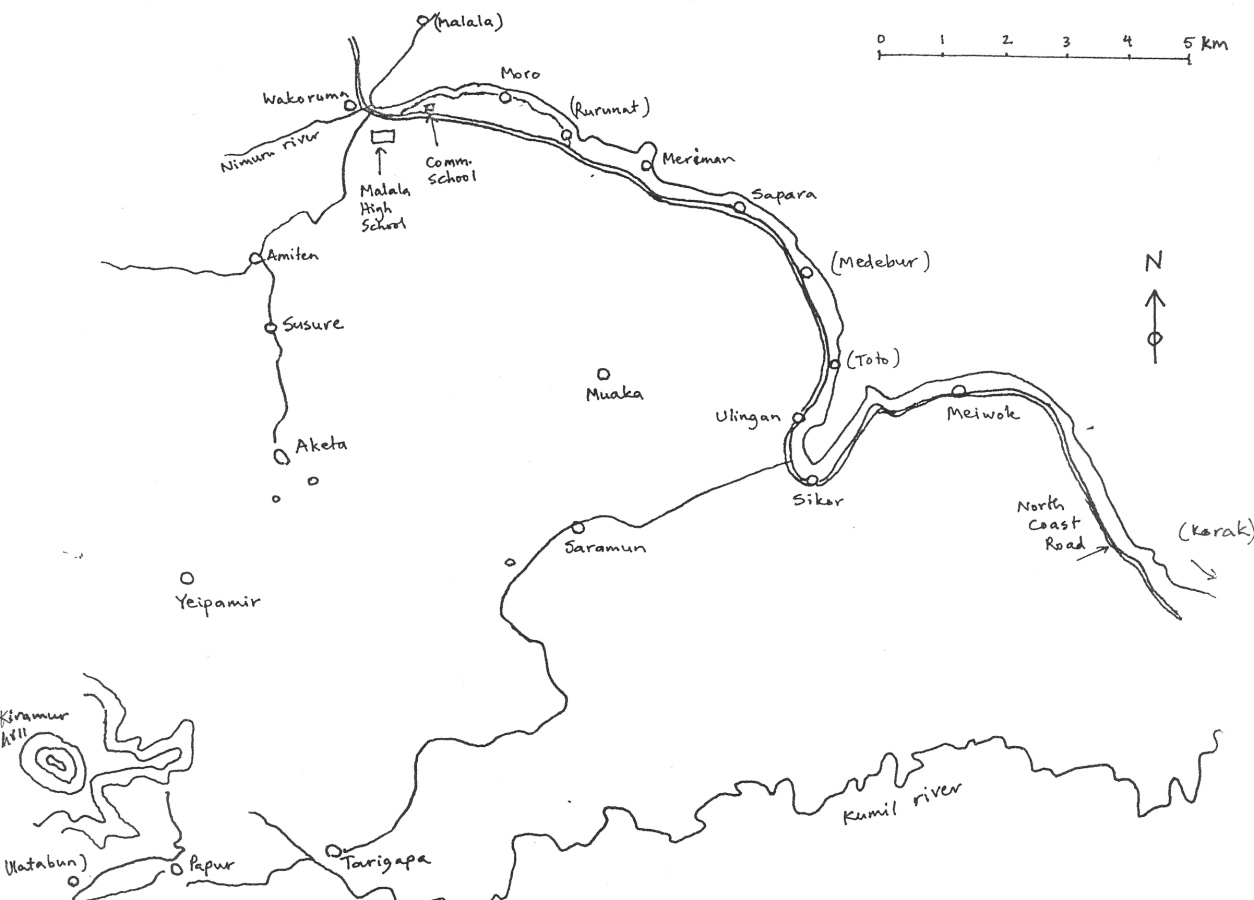
\includegraphics[width=\textwidth]{figures/1-mauwake_language_area_map.jpeg}
\end{figure}

Administratively the Mauwake people belong to the Bogia sub-province and the Almami (derived from the language names Alam--Mauwake--Miani) local level government area. 

There are four primary schools in the area, and one high school.  In all of these schools there are students from more than one language area. The Roman Catholic Church was instrumental in getting the schools started, and is still administering the Malala High School.  Nearly all of the children go to primary school, but the number of Mauwake students in the high school is not very high. Vernacular preschools were started in the whole Mauwake area in the early 1990s, but many of them have since changed into Tok Pisin preschools.

\subsection{On the history of the Mauwake people}
%\hypertarget{RefHeading18461935131865}
Until fairly recently, little was known about the pre-history of the Papuan-speaking people in Near Oceania (including New Guinea island, Bismarck Archipelago and the Solomon Islands), compared with the archaeological information available on the Austronesian-speaking people in the area. By the late 1990's it was established that human occupation on the northern coast of New Guinea island dated back to at least 40 000 years. There are signs of semi-domestication of some tree crops from 20 000 to 10 000 years ago, and of agriculture from about 10 000 years ago, roughly the same time that the Highlands valleys became more habitable after the end of the Ice Age \citep[xi-xvii]{Pawley2005a}. 

From the great diversity of the languages around Cape Croisilles area across Karkar Island, \citet[27]{Ross1996} hypothesizes that this probably is where the Croisilles linkage languages, including Mauwake (or its parent language), started spreading from.\footnote{See \sectref{sec:1.4.1} for a description of the genealogical affiliation. }  He does not provide any dates for the migrations.


Besides some traditional myths we have not been able to obtain stories telling about life earlier than the first half of the 20th century.  The majority of the Mauwake people agree that the language group has spread to the coast from inland, and they specify Aketa village as their place of origin. It is commonly believed that long ago the people of the Amiten village, now considered the ``heart area'' of the language by many speakers,spoke a different language, which has since disappeared. 

The hypothesis that the Mauwake people came from inland would at least partially explain the present language situation on the coast, where there are many languages scattered in a small geographical area. If at some point in history the coast did not have permanent inhabitants to defend it from intruders, it would have been easy for people migrating from various directions and speaking different languages to settle there. One cultural trait that points towards an earlier home area inland is that among the Mauwake speakers fishing is not as important as it is for some other language groups. The coastal villagers mainly catch fish for their own needs, and only occasionally take it to the local market if they happen to have surplus. Gardening, rather than fishing, is the important activity for them.

Possibly the first mention of the larger area where the Mauwake people live is given by the German \citet[338]{Hollrung1888}, who mentions ``the Tsimbin tribe'', meaning the people of Simbine village,\footnote{Situated 8 km from Moro village, and 5 km from the closest Mauwake village.} speaking the Maiani language which borders the Mauwake language area. \citet[964]{Holtker1937} calls Maiani and the related languages by the name ``M\'oando languages'' based on the word \textstyleEmphasizedWords{man} in those languages.  He also mentions Mauwake as ``Moro-Sapara-Ulingan'' -- picking names of three coastal villages -- as a language deviating from the M\'oando languages (ibid.). 

The written history of the Mauwake area itself began during the German colonial era (ca. 1884--1921) with the report of the killing of two Lutheran missionaries\footnote{The Rhenish Mission had planned to start the work in the area for some time, but it was blocked by the Neu-Guinea-Compagnie. The reason for the killing of the two missionaries, Wilhelm Scheidt and Friedrich Bösch, was never found out, but it is likely that the local people associated them with the Compagnie and feared that they were in fact planters coming to start plantations in their area \citep[106--107]{WagnerEtAl1986}} and an officer of the Neu-Guinea-Compagnie\footnote{The company had established a big coconut plantation further northwest on an island off Hatzfeldthafen in 1885. It developed quickly despite  various problems, but had to be abandoned completely in 1891 because of the hostility of the inhabitants of the area. Within 20 years the site was again covered by rainforest \citep[450--51]{Tranel1952}.} , as well as 14 accompanying native people, in Malala Bay in May 1891 (\citealt[454]{Tranel1952}, \citealt[106--109]{WagnerEtAl1986}).  After this the Lutheran church abandoned the plan to establish a mission station in the area, and founded one further southeast in the Bunabun area instead.

The Roman Catholic mission was then given the authority in 1891 to search the area between Ulingan and Bogia for suitable places for the mission \citep[8]{Duamba1996}.  The Ulingan-Sapara mission station was established in 1926, and a church big enough for a thousand people was built in Sapara village the same year \citep[21]{BrummEtAl1995}%Mihalic
.  A tsunami struck the coast in the morning of Christmas Eve, 1930, killing five people and destroying the new church and the priest's house.\footnote{Presumably the rest of the Sapara village was destroyed as well, as the church was probably the strongest building in the whole village.}  The mission station was moved to the Ulingan village and a new church was built on top of a hill there \citep[20--21]{Davies1999}. The Malala church was built in 1958 on land owned by the Moro villagers, and a high school started on the same compound in 1966 \citep[45]{BrummEtAl1995}%Mihalic
. Both the high school and all the community schools in the area were established by the Catholic Church.  Because of the many missionaries engaged in the work there the local people had a fair amount of contact with Westerners.

In the early years the priests were expected to learn the local language and to become familiar with the culture, especially religious beliefs \citep[25]{BrummEtAl1995}%Mihalic
. The liturgy and some preaching were done in Mauwake too, and a few hymns and prayers were composed in it. But whatever written materials there may have been, they were all lost in the Second World War \citep[3--4]{ZGraggen1971}.  And already in the 1930s Tok Pisin had started to replace the local languages as the official language for evangelization in the Catholic Church \citep[179]{BrummEtAl1995}%Mihalic
.  Especially in an area where five different languages are spoken along a 20 km stretch of the road, this is understandable.  

The Second World War had a profound influence on the area.  In December 1942 thousands of Japanese soldiers landed in Madang and Wewak (ibid. 37).  From Wewak the troops marched down towards Madang, and some of them settled in Ulingan.  They required the local men to help build bridges, and asked the people for food.  The women and also many men from the coastal villages fled to inland villages and to the rainforest, because they were scared of the soldiers.  They were suffering from a shortage of food, as they were not able to do their gardening in a normal way.  The Japanese apparently did not commit cruelties, as was the case in some other areas, and the relationship between them and the local people was uneasy but not hostile. When the Allied forces started to bomb the Japanese-occupied areas, the people had to keep hiding even more and were not even able to cook, as they were afraid that the smoke from their cooking fires might attract the pilots' attention and cause the area to be bombed.  A number of bombs were dropped in the Mauwake language area, and a few people died. 

Before the war, the missionaries were almost the only outsiders that the local people met, but during the war they had contact especially with Japanese but also with Allied soldiers.  After the war a number of young men went to work on plantations in different parts of the country or had other employment outside their home area, thus gaining knowledge of the wider world. The founding of Malala High School in 1966 and the completing of the North Coast Highway in the mid-70's further widened the people's horizons.

\subsection{Demography}   \label{sec:1.3.3} 


%\hypertarget{RefHeading18481935131865}


The inhabitants in the 15 Mauwake-speaking villages number about 4000;  the number is based on the census figures in 2000.  Not all of them speak the language, however, as most of the children now learn Tok Pisin as their first language.\footnote{Much of the contents of the sections \sectref{sec:1.3.3}-\sectref{sec:1.3.6} is based on the Mauwake background study written by Kwan Poh San in 1988.} 


The Mauwake speakers are not a uniform group socially or politically. The basic political unit is a village made up of a few clans. There is usually a main village, with some hamlets attached to it.  Recently there has been a tendency towards moving away from the main village and building small hamlets near the family's garden or coconut plot. 

A person's main responsibility is towards one's own family and clan. The basic unit is a nuclear family: parents and their children, either their own or adopted.  The society is patrilineal: kinship is traced through, and the inheritance handed down from, the father. Adoption is widespread and always takes place within extended family, usually the husband's side of the family.  Members of an extended family are expected to assist each other in various ways: providing food at feasts, helping to pay a debt, bride price or some other obligation, and looking after each other in general. The responsibilities towards one's clan are also strong but not quite as strong as to one's extended family.  Traditionally the clans used to own all the land, but planting coconuts, and later cocoa, changed the situation.  The use of garden land is still decided by the headmen (leaders) of each clan, but now there is rivalry even between members of the same clan about the existing coconut trees and about land where new coconut or cocoa trees can be planted.

Every clan has its own headman, and in earlier times the headman of the most prestigious clan also used to be the headman of the whole village. Decisions were based on consensus after discussions in the village meetings, but the final authority rested on the headmen.

After the establishment of the local level government system the authority of the headmen partly transferred to the local government member (\textstyleForeignWords{kaunsil}), to the magistrate and to the leader of the community work (\textstyleForeignWords{komiti}). The traditional authority structure has more or less broken down and since it has not been completely replaced by the new structure, this has given way to individualism and even disregard of any authority, especially among the young people. The Catholic Church is a somewhat cohesive force, but it has lost some of its authority with the social breakdown and also with the coming of other churches.

Each village has social ties with other, usually closely situated villages regardless of the language.  Many of the Mauwake villages have close interaction with non-Mauwake-speaking villages.  This has also resulted in extensive intermarrying between different language groups, which in the earlier times encouraged bilingualism or trilingualism, but which nowadays strengthens the use of Tok Pisin.

The six languages either bordering the Mauwake area, or inside it, are the Kaukombar\footnote{I am utilising \citegen{Ross2006} grouping here. For a discussion on the classification of the Madang languages, see {\S}\sectref{sec:1.4.1} below.} languages Maiani, Miani (Tani)\footnote{The names without parentheses are what the speakers prefer to use for their languages, the ones in parentheses are those used in linguistic literature especially by Z'Graggen and those utilising his data. Maiani and Miani are mentioned here as separate languages, but they can also be considered different dialects of one language.}  and Mala (Pay)\footnote{Mala has two distinct dialects, Mala and Alam. The latter is spoken in the two villages that have close contact with the Mauwake area.}, the Tibor language Mawak, the Korak-Waskia group language Amako (Korak), all of which are Trans New Guinea languages; the only Austronesian language is Beteka (Medebur), closely related to Manam language. None of these languages is dominant compared with the others.  The Mauwake speakers say that it used to be a prestigious language in the area, but I have not been able to confirm this with speakers of the other languages. Bi- and trilingualism used to be extensive in the whole area especially before the arrival of Tok Pisin. 


\subsection{Economy}
%\hypertarget{RefHeading18501935131865}
Subsistence farming is the main activity of the Mauwake people. They get most of their food and building materials from their own land.  Traditionally the main staple was taro, supplemented with yam, sweet potato and cooking bananas; sago was used particularly when little other food was available. Especially on the coast yam has recently been replacing taro as the main staple, because there is not enough land for slash-and-burn gardening required by taro. The traditional diet was very balanced, the basic meal including staples, vegetables and some smoked fish or meat, all cooked in coconut milk. Fruit eaten as snacks provided extra vitamins. Nowadays store-bought foods give variety to the diet but do not add much nutritional value, apart from tinned fish and meat, which provide some extra protein.

Hunting and fishing used to be important activities especially for men, but their significance has decreased. Wild pigs are getting scarce, and bandicoots are mainly hunted during the dry season.  As the Mauwake people have probably come from further inland, fishing has not been as important for them as for some other groups on the coast.  Both men and women do some fishing, but mainly for their own family's needs. 

Any garden produce, fish or bandicoots not needed by the family may be sold at the Malala market, which is the biggest one between Madang and Bogia, or at the smaller Ulingan market.  

For a long time coconut has been the main cash crop, but with the falling copra prices the people have diversified into growing cocoa, coffee\footnote{Growing coffee was given up later, because it is very labour-intensive and the \textstyleForeignWords{robusta} coffee grown in the lowlands fetches a very low market price.} and recently also vanilla.  The cash crops are transported to Madang to sell.  During the German colonial era tobacco was introduced in the area, and still in the 1930s Malala area was famous for its tobacco \citep[454]{Tranel1952}. Nowadays the people mainly grow it for their own use, and sell any extra at the local market.

The high school and a logging company provide employment for a few local men.  In the area where logging is done landowners also get some royalties from it.  Logging has caused controversy among the people.\footnote{The first logging company in the 1980s went bankrupt and the landowners received very little money for their timber.  Even with subsequent logging the benefits for the local people have been rather modest.} Many of the more educated men, and some women, now in their 40s and 50s have migrated into towns where they work as tradesmen, teachers, or in other occupations. 

\subsection{Cultural notes} 
%\hypertarget{RefHeading18521935131865}
In the traditional worldview the seen and the unseen are both important parts of the same universe.  The unseen world consists of different kinds of spirits: clan spirits and other spirits in nature (\textstyleStyleVernacularWordsItalic{inasina}), spirits of the recently dead (\textstyleStyleVernacularWordsItalic{kukusa}) and spirits of those who have died a long time ago (\textstyleStyleVernacularWordsItalic{sawur}). The spirits need to be treated with respect so that they will not harm but rather help the people.  Although the reliance on the spirits has decreased with the coming of Christianity, various rituals are still fairly widely practised to ensure the benevolence of the spirits, especially in connection with birth, death, sickness, hunting and gardening. 

Sickness is normally attributed to one's bad relations with other people or disregard of the spirits, the work of a sorcerer, or in some cases to ``natural causes''. Death is still commonly believed to be caused by sorcery.

Name taboos are a typical feature of the cultures in Oceania.  It is forbidden to call one's in-laws by name, or call anyone else by name who has the same name as the in-laws.  In the Mauwake culture both of the parents give a child the name of one of his or her own relatives, which the other parent naturally may not pronounce.  In addition to these two names, a child also receives a Christian name at baptism, and may be given other names as well.  Thus a person can have even five or six names, which are used by different people to call him or her.  And when the person gets married, all those names are forbidden for the in-laws to use.  They may use a kinship term or invent a nickname by which to address the person. In general, kinship terms are used widely both to address people and to refer to them.

Passing on the traditional culture and customs is hampered by the lessening use of the vernacular as well as the lack of interest especially among many young people. Grown-ups may deplore the situation, but there is little attempt to actively pass on the cultural heritage or to help the young generation to evaluate, appreciate and renew their own culture. 



\begin{sidewaysfigure}
%1-mauwake_kinship_system_cart.tex
\resizebox{\textwidth}{!}{
\begin{tikzpicture}

%	Naming Convention for this Picture
%	-------------------------------------
%	Text nodes are in normal letters
%	Shape notes are in ALLCAPS
%
%	Nodes are named 1-n depending on the distance to Ego 
%	Those left of Ego are preceeded by n, those right of Ego are followed by their indexical n

%	Margin conventions
%	Horizontally: Within children of the same parents: 1cm
%		-"-		  Within children of diff. parents: 1.75cm
%
%	Vertically:   Within children of diff. parents: 3.5cm

%Padding for family members
[every rectangle node/.style={inner sep=6pt}]
%circle size, globally
% [every circle node/.sytle={minimum size=.6cm}] Doesn't work, why?

%Ego
\node at (0,0) [rectangle, draw] (ego) {Ego};
\node [above=.1cm of ego,regular polygon, regular polygon sides=3, draw, fill=gray] (EGO) {}; 
%Brother of Ego
\node [left=3cm of ego, rectangle, draw] (1br) {Br};
\node [above=.1cm of 1br, regular polygon, regular polygon sides=3, draw] (1BR) {};
%Sister of Ego
\node [right=3cm of ego, rectangle, draw] (z1) {Z};
\node [above=.1cm of z1, circle, minimum size=.6cm, draw] (Z1) {};

% Ego's cousins on their mother's side
\node [right=1.75cm of z1, rectangle, draw] (br1) {Br};
\node [above=.1cm of br1, regular polygon, regular polygon sides=3, draw] (BR1) {};
\node [right=1cm of br1, rectangle, draw] (z2) {Z};
\node [above=.1cm of z2, circle, minimum size=.6cm, draw] (Z2) {};

\node [right=1.75cm of z2, rectangle, draw] (co1) {Co};
\node [above=.1cm of co1, regular polygon, regular polygon sides=3, draw] (CO1) {};
\node [right=1cm of co1, rectangle, draw] (co2) {Co};
\node [above=.1cm of co2, circle, minimum size=.6cm, draw] (CO2) {};

% Ego's cousins on their mother's side
\node [left=1.75cm of 1br, rectangle, draw] (1z) {Z};
\node [above=.1cm of 1z, circle, minimum size=.6cm, draw] (1Z) {};
\node [left=1cm of 1z, rectangle, draw] (2br) {Br};
\node [above=.1cm of 2br, regular polygon, regular polygon sides=3, draw] (2BR) {};

\node [left=1.75cm of 2br, rectangle, draw] (1co) {Co};
\node [above=.1cm of 1co, circle, minimum size=.6cm, draw] (1CO) {};
\node [left=1cm of 1co, rectangle, draw] (2co) {Co};
\node [above=.1cm of 2co, regular polygon, regular polygon sides=3, draw] (2CO) {};

% Ego's parents
\node [above left=3.5cm and .5cm of ego, rectangle, draw] (1fr) {Fr};
\node [above=.1cm of 1fr, regular polygon, regular polygon sides=3, draw] (1FR) {};
\node [above right=3.5cm and .5cm of ego, rectangle, draw] (mo1) {Mo};
\node [above=.1cm of mo1, circle, minimum size=.6cm, draw] (MO1) {};

% Marriage smyol of Ego's parents
\node [above=3.5cm of EGO] (1frmo1) {\huge{=}};

% Ego's Aunties and Uncles
\node [above=3.5cm of br1, rectangle, draw] (fr1) {Fr};
\node [above=.1cm of fr1, regular polygon, regular polygon sides=3, draw] (FR1) {};
\node [right=1cm of fr1, rectangle, draw] (mo2) {Mo};
\node [above=.1cm of mo2, circle, minimum size=.6cm, draw] (MO2) {};
\node at ($(MO2) !.5! (FR1)$) (fr1mo2) {\huge{=}};

\node [above=3.5cm of co1, rectangle, draw] (un1) {Un};
\node [above=.1cm of un1, regular polygon, regular polygon sides=3, draw] (UN1) {};
\node [right=1cm of un1, rectangle, draw] (au1) {Au};
\node [above=.1cm of au1, circle, minimum size=.6cm, draw] (AU1) {};
\node at ($(UN1) !.5! (AU1)$) (un1au1) {\huge{=}};

\node [above=3.5cm of 2br, rectangle, draw] (2fr) {Fr};
\node [above=.1cm of 2fr, regular polygon, regular polygon sides=3, draw] (2FR) {};
\node [right=1cm of 2fr, rectangle, draw] (1mo) {Mo};
\node [above=.1cm of 1mo, circle, minimum size=.6cm, draw] (1MO) {};
\node at ($(2FR) !.5! (1MO)$) (2fr1mo) {\huge{=}};

\node [above=3.5cm of 2co, rectangle, draw] (1un) {Un};
\node [above=.1cm of 1un, regular polygon, regular polygon sides=3, draw] (1UN) {};
\node [right=1cm of 1un, rectangle, draw] (1au) {Au};
\node [above=.1cm of 1au, circle, minimum size=.6cm, draw] (1AU) {};
\node at ($(1UN) !.5! (1AU)$) (1un1au) {\huge{=}};

% Ego's Grandparents
% ... on their father's side
\node [above=3.5cm of 2fr, rectangle, draw] (1grfa) {GrFa};
\node [above=.1cm of 1grfa, regular polygon, regular polygon sides=3, draw] (1GRFA) {};
\node [right=1cm of 1grfa, rectangle, draw] (1grmo) {GrMo};
\node [above=.1cm of 1grmo, circle, minimum size=.6cm, draw] (1GRMO) {};
\node at ($(1GRFA) !.5! (1GRMO)$) (1grfa1grmo) {\huge{=}};

% ... on their mother's side
\node [above=3.5cm of fr1, rectangle, draw] (grfa1) {GrFa};
\node [above=.1cm of grfa1, regular polygon, regular polygon sides=3, draw] (GRFA1) {};
\node [right=1cm of grfa1, rectangle, draw] (grmo1) {GrMo};
\node [above=.1cm of grmo1, circle, minimum size=.6cm, draw] (GRMO1) {};
\node at ($(GRFA1) !.5! (GRMO1)$) (grfa1grmo1) {\huge{=}};

% Ego's children
\node [below left=3.5cm and .5cm of ego, regular polygon, regular polygon sides=3, draw] (1SO) {};
\node [below=.1cm of 1SO, rectangle, draw] (1so) {So};
\node [right=1cm of 1so, rectangle, draw] (da1) {Da};
\node [above=.1cm of da1, circle, minimum size=.6cm, draw] (DA1) {};

% Ego's Nephews and Niece
\node [left=1.75cm of 1so, rectangle, draw] (1da) {Da};
\node [above=.1cm of 1da, circle, minimum size=.6cm, draw] (1DA) {};
\node [left=1cm of 1da, rectangle, draw] (2so) {So};
\node [above=.1cm of 2so, regular polygon, regular polygon sides=3, draw] (2SO) {};

\node [right=1.75cm of da1, rectangle, draw] (ne1) {Ne};
\node [above=.1cm of ne1, regular polygon, regular polygon sides=3, draw] (NE1) {};
\node [right=1cm of ne1, rectangle, draw] (ne2) {Ne};
\node [above=.1cm of ne2, circle, minimum size=.6cm, draw] (NE2) {};

% Ego's female Cousin's children 

\node [below left=3.5cm and .5cm of 1co, regular polygon, regular polygon sides=3, draw] (3SO) {};
\node [below=.1cm of 3SO, rectangle, draw] (3so) {So};
\node [right=1cm of 3so, rectangle, draw] (2da) {Da};
\node [above=.1cm of 2da, circle, minimum size=.6cm, draw] (2DA) {};


% In-Generation Connections

% Usage of in-generation connections:
% We are using Node Coordinate System, see Section 13.2.3 of the PGF manual
% \draw (node cs:name=NAME, anchor=north) |- +(0,.5) -| (node cs:name=2ndNAME);
% note: We use anchor=north in order to prevent PGF from choosing any other, just in case. We will probably not need it in the second node, though
% note 2: +(0,.5) is a relative position, meaning .5 vertical positive change
% |- means: Go vertical first and then horizontally

% Ego & their immediate Br & Z
\draw (node cs:name=EGO, anchor=north) |- +(0,.5) -| (node cs:name=Z1);
\draw (node cs:name=EGO, anchor=north) |- +(0,.5) -| (node cs:name=1BR);

% Ego's cousins on their mother's side
\draw (node cs:name=BR1, anchor=north) |- +(0,.5) -| (node cs:name=Z2) node [pos=.25] (MBR1Z2) {};
\draw (node cs:name=CO1, anchor=north) |- +(0,.5) -| (node cs:name=CO2) node [pos=.25] (MCO1CO2) {};

% Ego's cousins on their father's side
\draw (node cs:name=1Z, anchor=north) |- +(0,.5) -| (node cs:name=2BR) node [pos=.25] (M1Z2BR) {};
\draw (node cs:name=1CO, anchor=north) |- +(0,.5) -| (node cs:name=2CO) node [pos=.25] (M1CO2CO) {};

% Ego's fathers and his brother and sister
\draw (node cs:name=1FR, anchor=north) |- +(0,.5) -| (node cs:name=1AU);
\draw (node cs:name=1FR, anchor=north) |- +(0,.5) -| (node cs:name=2FR) node [pos=.25] (M1FR2FR);

% Ego's mother and her brother and sister
\draw (node cs:name=UN1, anchor=north) |- +(0,.5) -| (node cs:name=MO2);
\draw (node cs:name=UN1, anchor=north) |- +(0,.5) -| (node cs:name=MO1) node [pos=.25] (MUN1NO1) {};

% Ego's children and nephews/nieces
\draw (node cs:name=1SO, anchor=north) |- +(0,.5) -| (node cs:name=DA1) node [pos=.25] (M1SODA1) {};
\draw (node cs:name=NE1, anchor=north) |- +(0,.5) -| (node cs:name=NE2) node [pos=.25] (MNE1NE2) {}; % relative positioning. Not sure why it's 1/4, tough. 
\draw (node cs:name=2SO, anchor=north) |- +(0,.5) -| (node cs:name=1DA) node [pos=.25] (M2SO1DA) {};
\draw (node cs:name=3SO, anchor=north) |- +(0,.5) -| (node cs:name=2DA) node [pos=.25] (M3SO2DA) {};


% Between-Generation Connections

% The old way was \draw (node cs:name=grfa1grmo1, anchor=south) -- ($(grfa1grmo1)-(0,3.225)$); This was extremly messy.
% The new way is to use |- and a seperate node on the |--| specified above. A little tricky, but it should be reliable.


\draw (node cs:name=1frmo1, anchor=south) -- (node cs:name=EGO, anchor=north);
\draw (node cs:name=fr1mo2, anchor=south) |- (node cs:name=MBR1Z2, anchor=center);
\draw (node cs:name=un1au1, anchor=south) |- (node cs:name=MCO1CO2, anchor=center);
\draw (node cs:name=2fr1mo, anchor=south) |- (node cs:name=M1Z2BR, anchor=center);
\draw (node cs:name=1un1au, anchor=south) |- (node cs:name=M1CO2CO, anchor=center);
\draw (node cs:name=grfa1grmo1, anchor=south) |- (node cs:name=MUN1NO1, anchor=center);
\draw (node cs:name=1grfa1grmo, anchor=south) |- (node cs:name=M1FR2FR, anchor=center);
\draw (node cs:name=1co, anchor=south) |- (node cs:name=M3SO2DA, anchor=center);
\draw (node cs:name=ego, anchor=south) |- (node cs:name=M1SODA1, anchor=center);

\draw (node cs:name=1br, anchor=south) |- (node cs:name=M2SO1DA, anchor=center); %This is precise
\draw (node cs:name=z1, anchor=south) |- (node cs:name=MNE1NE2, anchor=center); %This is precise


\end{tikzpicture}
}
\caption{Mauwake kinship system chart}
\label{fig:1:kinship}
\end{sidewaysfigure}
 



\subsection{Mauwake kinship system} \label{sec:1.3.6}
%\hypertarget{RefHeading18541935131865}
The kinship system of the Mauwake people is a slightly modified Iroquis system. Both gender and generation are important, but also the distinction of parental siblings of the opposite sex (Chart 1). One's father's brother is also called \textstyleStyleVernacularWordsItalic{auwa} `father' and his wife is \textstyleStyleVernacularWordsItalic{aite} `mother'; likewise one's mother's sister is also `mother' and her husband is `father'. But mother's brother is called \textstyleStyleVernacularWordsItalic{yaaya} `uncle', and his wife is \textstyleStyleVernacularWordsItalic{paapan} `aunt'; father's sister is also `aunt' and her husband is `uncle'. The term `father' is used for the following as well: one's own father's cross-cousins, one's father-in law and, for a female, elder sister's husband. Two generations up from self the grandparents are distinguished by gender: \textstyleStyleVernacularWordsItalic{kae} `grandfather' and \textstyleStyleVernacularWordsItalic{kome} `grandmother', but two generations down all the grandchildren are called \textstyleStyleVernacularWordsItalic{iimasip} `grandchild'. 

In one's own generation there are two sets of terms for brothers and sisters. Their use  depends on whether relative age or gender is in focus: \textstyleStyleVernacularWordsItalic{paapa} `older sibling' and \textstyleStyleVernacularWordsItalic{aamun} `younger sibling' are used for siblings of either sex, whereas \textstyleStyleVernacularWordsItalic{yomokowa} `brother'  and \textstyleStyleVernacularWordsItalic{ekera} `sister' are gender-bound terms. The latter are more commonly used by siblings of the opposite sex than by those of the same sex. All the parallel cousins are also considered one's siblings, whereas one's cross-cousins, the children of the `uncles' and `aunts', are called \textstyleStyleVernacularWordsItalic{yomar/emar} `cousin', a term used for either sex.

One generation down from self, one's children include not only one's own sons (\textstyleStyleVernacularWordsItalic{muuka}) and daughters (\textstyleStyleVernacularWordsItalic{wiipa}), but also those of one's siblings of the same sex, \textstyleEmphasizedWords{and} those of one's cross-cousins. For the sons and daughters of one's siblings of the opposite sex there is a single term, \textstyleStyleVernacularWordsItalic{eremena} `nephew/niece'. Most of the terms for kin relations are inalienably possessed nouns (\sectref{sec:3.2.4}). 

Mother's brother is a particularly important relative for performing rites of passage like initiation, marriage and funeral. When a person dies, his/her maternal uncle, together with the deceased person's male cross-cousins, is responsible for burying him/her and distributing his/her possessions.\footnote{For an older person whose uncles have already died, nephews (= sons of the siblings of opposite sex) take their place among these men..} These men are called \textstyleStyleVernacularWordsItalic{weria} men.  \textit{Weria} means `planting stick', and the term is used as a metaphor for burial.\footnote{It is not unusual to have the same verb for `burying' and `planting' in Papuan languages, but in Mauwake they are different.} An uncle also has an important function as a mediator, if his nephew or niece has serious problems with his/her nuclear family. Although father's sister's husband is also called an `uncle', he does not have a similar role to that of mother's brother.  

\section{The Mauwake language}
%\hypertarget{RefHeading18561935131865}
\subsection{Genealogical affiliation and previous research}\label{sec:1.4.1}
%\hypertarget{RefHeading18581935131865}
The name \emphs{Mauwake} means `what?'\footnote{Actually it consists of the question word \textit{mauwa} `what' and the contrastive focus clitic -\textit{ke}.}  The Mauwake speakers themselves identify the language by this name, and the speakers of the related Kaukombaran languages use corresponding names to call their own languages.  The people have a myth in which the spirit Turamun gives each group their land area, their main staple as well as their language, and the language name originates in this myth.

Before our taking residence in Moro village in 1978, there was only very sketchy research done on the Mauwake language, just enough to classify it.\footnote{\citet{Capell1952}, and following him \citet{VoegelinEtAl1965}, \citet{Greenberg1971}, then \citet{ZGraggen1971,ZGraggen1975a}, \citet{Wurm1975,Wurm1982} and \citet{Hattori1981}.} The name Ulingan was taken from the main mission station in the area, although that is not how the speakers themselves call their language. Sometimes the alternative name Mawake is given in brackets in the earlier language lists.  

Mauwake is a Papuan language. `Papuan' is just a cover term for a number of genetically unrelated language families, which are not Austronesian and are spoken in the New Guinea region.\footnote{The name Papuan has been criticized (\citealt{Capell1969}, \citealt{Haiman1979}), but it is widely used instead of its alternative, non-Austronesian.} The Papuan languages consist of several unrelated language families, the biggest of which is the Trans New Guinea (\textsc{tng}) family.  


\begin{figure}
\caption{New Guinea island language map \citep[34 Map~2]{Ross2005}}
\label{map:2:NewGuineamap}
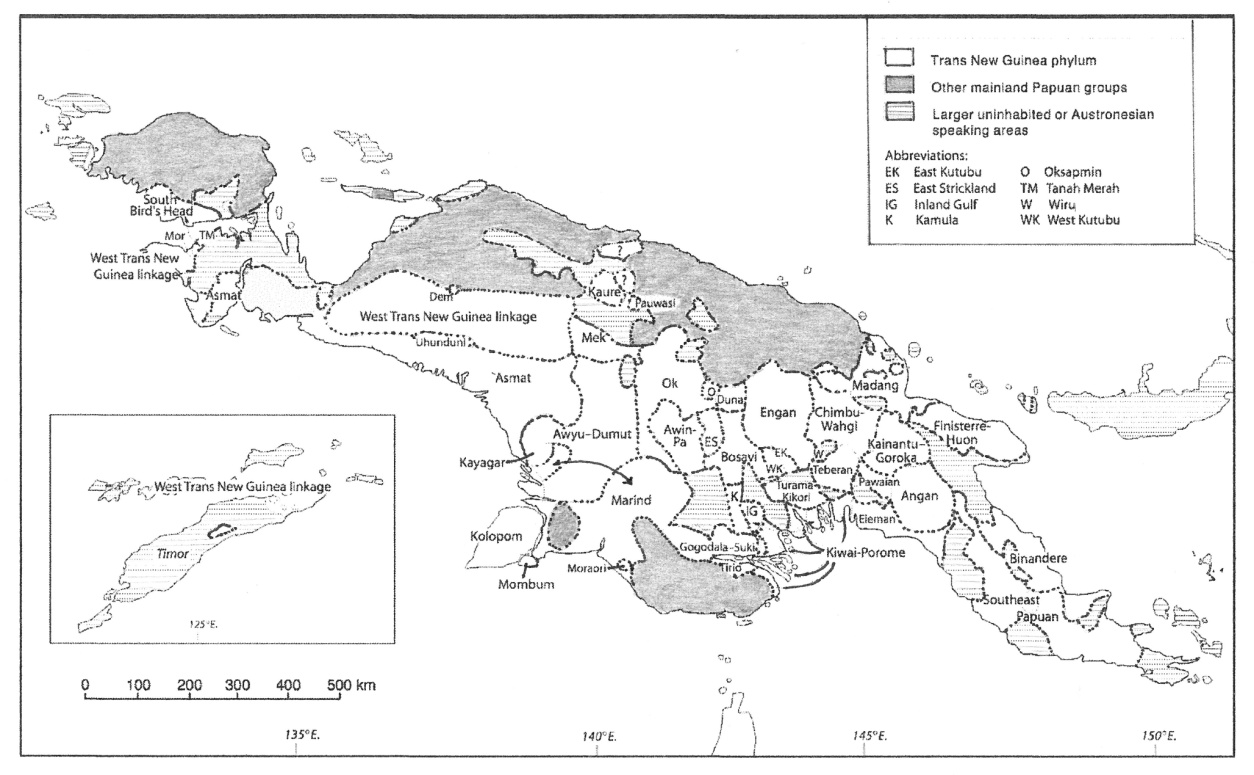
\includegraphics[width=\textwidth]{figures/1-new_guinea_island_language_map.jpeg}
\end{figure}

The Trans New Guinea hypothesis was originally put forward by \citet{McElhanonEtAL1970} to account for the similarities between the Finisterre-Huon languages on the one hand, and Central and South New Guinea Stock languages on the other. Later \citet{Wurm1975} argued that a great number of additional languages belong to the phylum.  Much of the work relied on lexico-statistical rather than more rigorous application of the standard comparative method, and because many of the claims are not well substantiated, the whole \textsc{tng} hypothesis received a fair bit of criticism (\citealt{Lang1976}, \citealt{Haiman1979}, \citealt{Foley1986}, \citealt{Pawley1995}).

Most of the classificatory work done on the languages of Madang Province is based on \citet{ZGraggen1971,ZGraggen1975} groundbreaking research.  According to \citegen{Wurm1975} classification following the language family tree model of lexicostatistics, Mauwake\footnote{In \citegen{ZGraggen1980} listing Mauwake has the code F2, and the ISO 639--3 code for the language is mhl.} belongs to the Madang-Adelbert Range sub-family, Adelbert Range superstock, Pihom stock, and Kumilan\footnote{\citet{ZGraggen1971} initially called the family Ubean, possibly based on the language names Ulingan and Bepour, but later (1975) changed the name into Kumilan based on the name of the Kumil river.} language family together with two very small languages, Bepour and Moere. 




\begin{figure}
\caption{Wurm's grouping of Madang-Adelbert languages \citep [Map~3]{Ross1996}}
\label{map:3:MadangWurm}
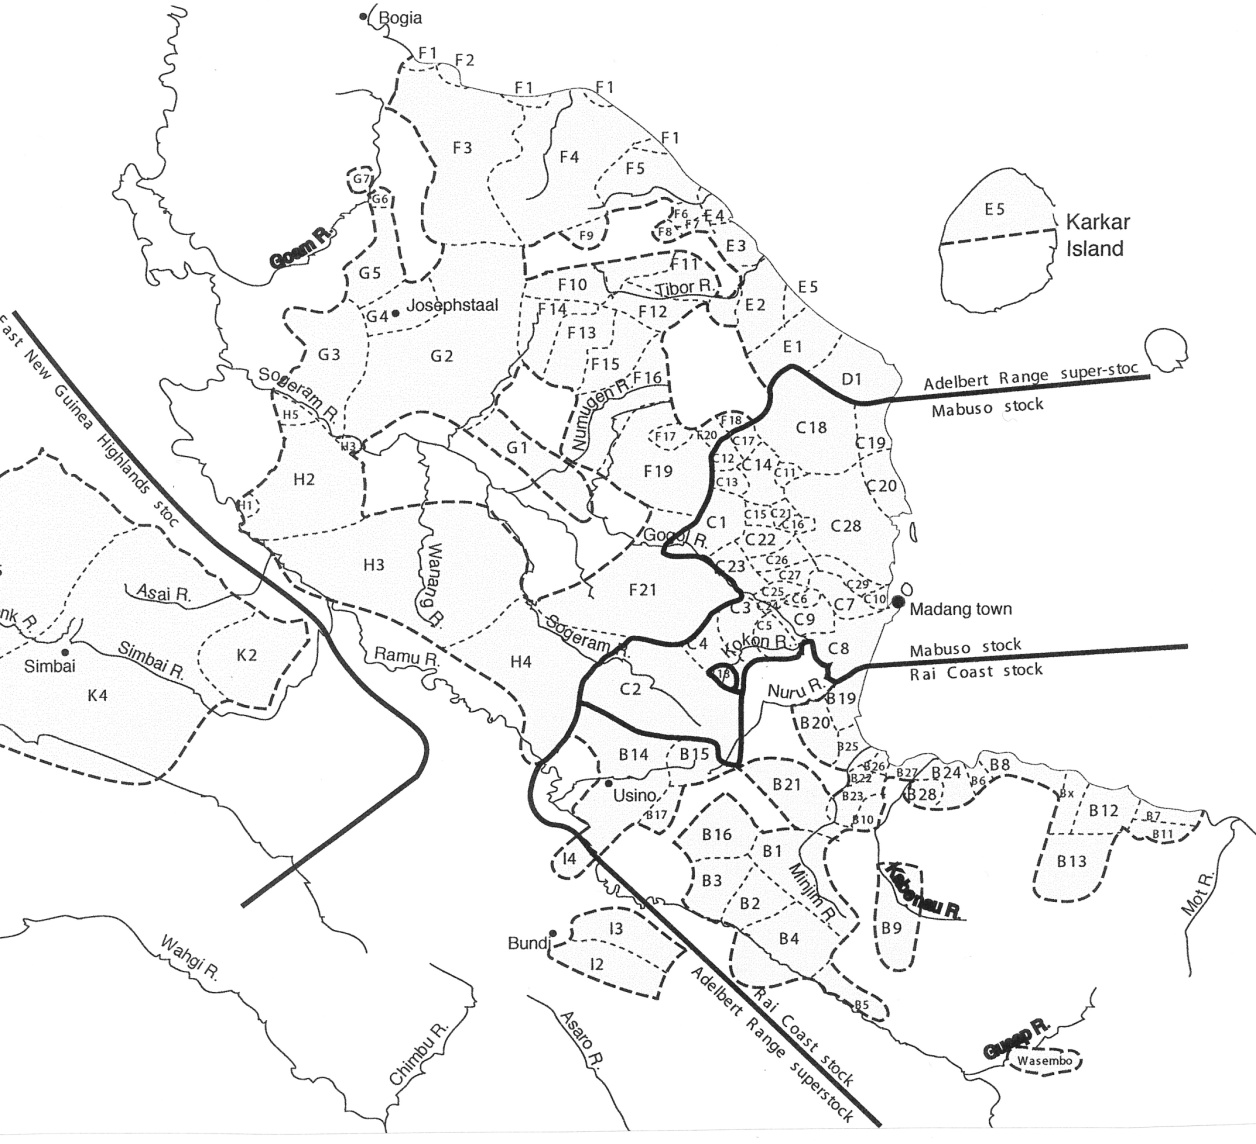
\includegraphics[width=\textwidth]{figures/1-wurms_grouping_of_madang_adelbert_languages.jpeg}
\end{figure}

For nearly two decades there was practically no comparative linguistics done on Papuan languages.  But in the early 1990s more detailed research started on the Madang-Adelbert Range languages, now renamed the Madang group, and later on other \textsc{tng} languages as well \citep{Pawley1998}. As a result of that research \citet{Pawley1995, Pawley2001} and \citet{Ross1995} came to the conclusion that the Trans New Guinea hypothesis is workable but needs modification. They also concluded that the Madang group definitely is part of the Trans New Guinea language family. According to their new classification Mauwake belongs to the Trans New Guinea family, the Madang group and the Croisilles linkage of languages. \citet[21--25]{Ross1996} also discusses the relationships between the various languages within the Croisilles subgroup, using the term \textstyleEmphasizedWords{Kumil} (Z'Graggen's  \textstyleEmphasizedWords{Kumilan} ) for the family including Mauwake, and \textstyleEmphasizedWords{Kaukombar} (Z'Graggen's \textstyleEmphasizedWords{Kaukombaran} ) for the four languages closest to the Kumil languages. He also does some regrouping within the families based on the pronoun  forms in the languages.  In the Kumil group he includes not only Mauwake, Bepour and Moere, but also the languages Musar and Bunabun. 



\begin{figure}
\caption{Ross' 1996 grouping of Madang-Adelbert languages \citep[Map~4]{Ross1996}}
\label{map:4:MadangRoss}
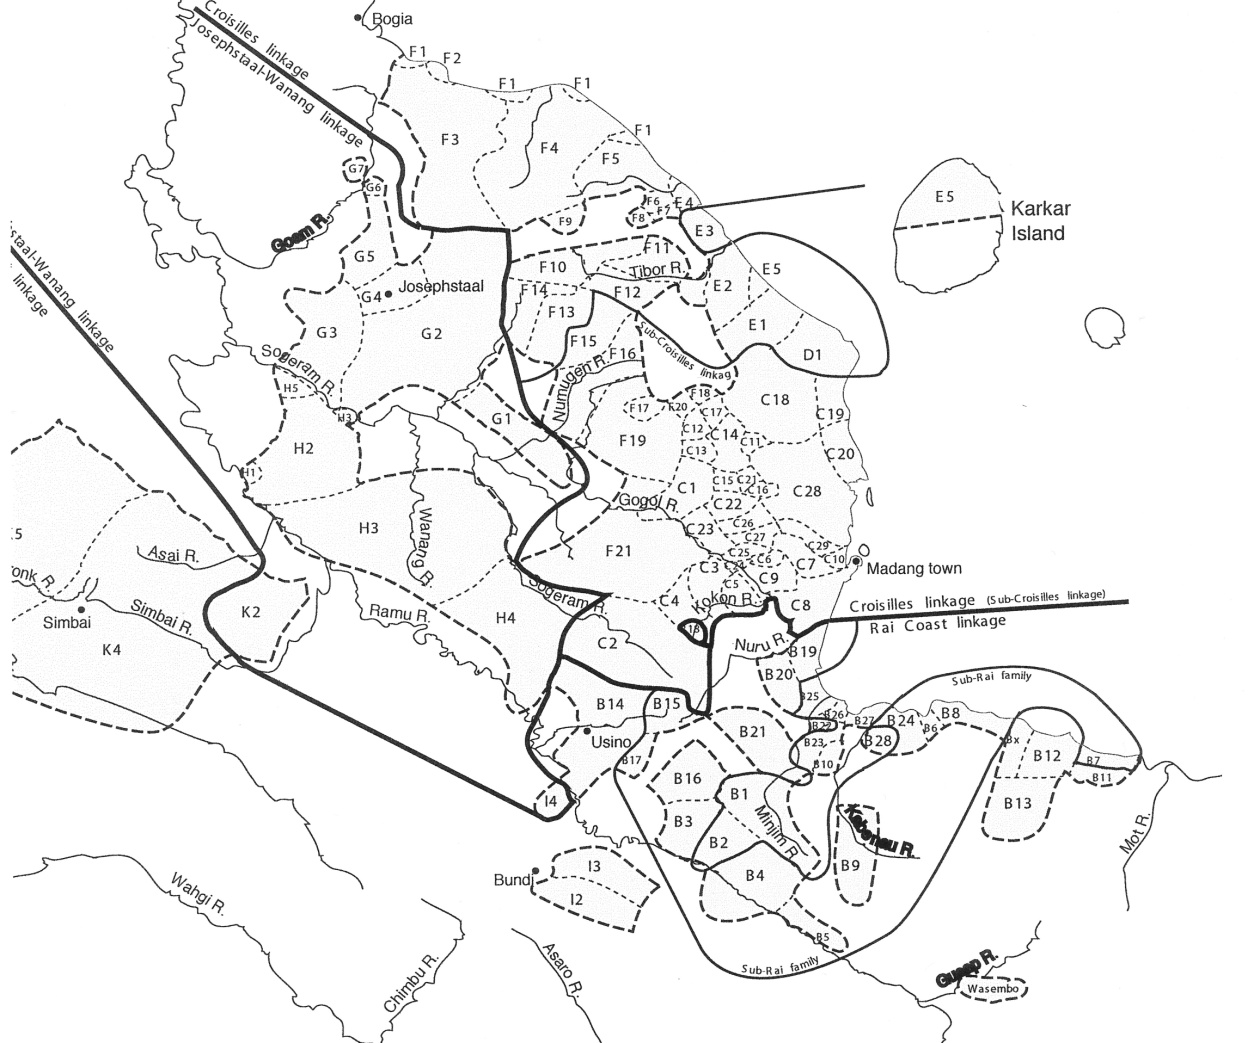
\includegraphics[width=\textwidth]{figures/1-ross_grouping_of_Madang_Adelbert_languages_map.jpeg}
\end{figure}

Apart from Z'Graggen's survey no other linguistic study of any depth has been carried out on the Mauwake language except what has been done by Kwan Poh San and myself (\citealt{Kwan1980, Kwan1983, Kwan1988, Kwan1989, Kwan2002}; \citealt{Jarvinen1980,Jarvinen1988a,Jarvinen1988b,Jarvinen1989,Jarvinen1990,Jarvinen1991}; \citealt{JarvinenEtAl2001}, and \citealt{Berghall2006}.)  The grammatical work published on related languages includes Reesink's grammar of \citet{Usan1987}, MacDonald's grammar of \citet{Tauya1990} and Ross and Paol's grammar of \citet{Waskia1978}. Two grammars in manuscript form that were also used for reference are Maia grammar by Barbara Hardin and Bargam grammar by Mark Hepner. Both are available electronically and in the \textsc{sil-png} library, Ukarumpa.

The \textsc{iso}-639 code for Mauwake, based on \citet{Grimes2000}, is mhl, and the Glottolog code is mauw1238 (glottolog.org).

\subsection{Typological overview of morphological and syntactic features}
%\hypertarget{RefHeading18601935131865}
In this section, morphological and syntactic characteristics of the Mauwake language are discussed in relation to the typology of Papuan/Trans New Guinea languages and to the universal word order\footnote{As \citet[72]{Dixon2009} notes, ``word order'' here should be called ``(clausal) constituent order'', as it is the ordering of constituents that the typology is based on rather than that of individual words.}  typology.  To some extent these two overlap, as \textsc{tng} languages typically are also \textsc{sov} languages.

\paragraph[Mauwake as a Trans New Guinea language]{Mauwake as a Trans New Guinea language}
%\hypertarget{RefHeading18621935131865}
Mauwake has many features typical of both Papuan languages in general and Trans New Guinea languages in particular. 

The \textstyleEmphasizedWords{{phonology}} of the language is simple: there are five vowel and fourteen consonant phonemes, and only a few of them have more than one allophone.  Morphology is quite transparent, so there is very little morphophonology.

The \textstyleEmphasizedWords{{basic}} \textstyleEmphasizedWords{{order of clausal constituents}} is verb-final. In neutral clauses with both subject and object the order is \textsc{sov} \REF{ex:1:x656}, but it changes into \textsc{osv} when the object is fronted \REF{ex:1:x657} as a theme (9.1)\todo{right number?}.  Adverbials are somewhat less constrained in their ordering. It is also very common to have the verb as the only element in a clause \REF{ex:1:x659}. 

\ea%x656
\label{ex:1:x656}
\gll [Ona  emeria  nain=ke]\textsubscript{S} [maa]\textsubscript{O} wafur-a-k. \\
 3s.\textsc{gen} woman  that1=\textsc{cf}  thing  throw-\textsc{pa}-3s \\
\glt `His wife threw things.'
\z


\ea%x657
\label{ex:1:x657}
\gll [Wiipa  nain]\textsubscript{O} [eka=ke]\textsubscript{S} mu-o-k. \\
 daughter  that1  water=\textsc{cf} swallow-\textsc{pa}-3s     \\
\glt `The daughter was swallowed by the water.'
\z


\ea%x659
\label{ex:1:x659}
\gll Uruf-a-m. \\
 see-\textsc{pa}-1s     \\
\glt `I saw it.'
\z


In \textstyleEmphasizedWords{{complex sentences}} the subordinate clause usually precedes the main clause.  Thus the reason/cause precedes the result/effect, in conditional sentences protasis precedes the apodosis, and in intention/purpose sentences the intention precedes the expected result. When the reason follows the result, it is a very marked order.

Mauwake is clearly a nominative-accusative type language, rather than ergative-absolutive. The agent of a transitive verb \REF{ex:1:x1523} is marked in the same way as the actor of an intransitive verb \REF{ex:1:x1524}, and most experiential verbs have the experiencer as a nominative subject \REF{ex:1:x1525}.

\ea%x1523
\label{ex:1:x1523}
\gll Yo  mauw-owa  nia  asip-i-yem. \\
 1s.\textsc{unm}  work-\textsc{nmz}  2p.\textsc{acc}  help-\textsc{Np}-\textsc{pr}.1s     \\
\glt `I help you with work.'
\z


\ea%x1524
\label{ex:1:x1524}
\gll Yo  koka=pa  ik-e-m. \\
1s.\textsc{unm}  jungle=\textsc{loc}  be-\textsc{pa}-1s      \\
\glt `I was in the jungle.'
\z


\ea%x1525
\label{ex:1:x1525}
\gll Yo  wailal-i-yem  a. \\
 1s.\textsc{unm}  hunger-\textsc{Np}-\textsc{pr}.1s  oh     \\
\glt `Oh, I'm hungry.'
\z


\textstyleEmphasizedWords{{Verb morphology}} in Mauwake is extensive, even if not as extensive and complex as in some other Papuan languages. The morphology is agglutinative, and  affixation is mostly very transparent.  Suffixes are used for subject, tense and aspect, benefactive, distributive, causative and counterfactual marking. Prefixing is used very little, only for reduplication and to form verbs referring to bringing and taking. It is possible to have several derivational and inflectional affixes in one verb, as shown by the elicited example \REF{ex:1:x664}, but in actual usage this is rare.


\ea%x664
\label{ex:1:x664}
\gll Muuka  wia \textstyleEmphasizedVernacularWords{arim-ow-omak-om-ek-a-k}. \\
 son  3p.\textsc{acc}  grow-\textsc{caus}-\textsc{distr/pl}-\textsc{ben}-\textsc{bnfy1.\textsc{cntf}-pa}-3s     \\
\glt `(S)he would have brought up (many) sons for me.'
\z


Mauwake has a clear three-tense system (\sectref{sec:3.8.3.4}). Even though the tense suffixes only distinguish between past and non-past, the distinction between present and future shows in the subject suffixes, which are different for these two tenses.  Aspect marking is optional (\sectref{sec:3.8.5.1.1}).  The auxiliary follows the main verb. There is no passive form in verbs.

A very typical feature in the Papuan languages is a difference between final (\sectref{sec:3.8.3.4}) and medial verbs (\sectref{sec:3.8.3.5}). The former are finite verbs with full inflection for tense and subject number and person, and the most typical position for them is at the end of a declarative sentence. The medial verbs indicate whether the subject of a clause is the same as \REF{ex:1:x662}, or different from \REF{ex:1:x663}, that of the following clause. The same-subject forms also indicate whether the action of the second verb is simultaneous with that of the first verb, or sequential \REF{ex:1:x662} in relation to it. Medial clauses (\sectref{sec:8.2}) are coordinate with, but also dependent on, the following clause. Because of the existence and extensive use of medial clauses, temporal subordinate clauses (\sectref{sec:8.3.3.1}) are used very little in Mauwake.\footnote{Medial clauses in Papuan languages are often translated with temporal subordinate clauses in other languages, even if they are not subordinate in the original language.}

\ea%x662
\label{ex:1:x662}
\gll Owowa  ek-\textstyleEmphasizedVernacularWords{ap},  wailal-\textstyleEmphasizedVernacularWords{ep}  akia  ik-e-k. \\
village  go-\textsc{ss.seq} be.hungry-\textsc{ss.seq} banana  roast-\textsc{pa}-3s      \\
\glt `He went to the village, was hungry and roasted bananas.'
\z

%\ea%x663
%\label{ex:1:x663}
%\gll \emphs{Mik-}\textstyleEmphasizedVernacularWords{amkun}\emphs{  me  um-o-k,  wiowa  onaiya  ikiw-em-ik}%-\textstyleEmphasizedVernacularWords{eya}. \\
%spear-1s/p.DS  not  die-PA-3s  spear  with  go-SS\textsc{sim}-be-2/3s.DS
%\emphs{Olas=ke  war-e-k}
%Olas=CF  kill-PA-3s     \\
%\glt`When I speared it, it didn't die, (but) as it was going with the spear Olas killed it.'
%\z

 
\ea%x663
\label{ex:1:x663}
\gll Mik-\textstyleEmphasizedVernacularWords{amkun}   me  um-o-k,  wiowa  onaiya  ikiw-em-ik-\textstyleEmphasizedVernacularWords{eya}. Olas=ke  war-e-k\\
spear-1s/p.\textsc{ds}  not  die-\textsc{pa}-3s  spear  with  go-\textsc{ss.sim}-be-2/3s.\textsc{ds} Olas=\textsc{cf}  kill-\textsc{pa}-3s\\
\glt`When I speared it, it didn't die, (but) as it was going with the spear Olas killed it.'
\z


Medial verbs are also used in tail-head linkage (\sectref{sec:8.2.3.5}), another strategy common in Papuan languages. The last verb of a sentence is repeated in the first clause of the next sentence, but usually in medial form.  In spoken Mauwake this recapitulation device is used to indicate actions that continue on the story line without a major break, but since the development of the written language the tail-head linkage is losing this function and is getting a new function as a  marker of the climax in the story.

Another typical feature of many Papuan languages is the lack of a large inventory of verb stems \citep[127]{Foley1986}. An extreme case is Kalam with its less than 100 verb stems; consequently, Kalam needs to use serial verb and adjunct plus verb constructions for most actions \citep[336--337]{Pawley1987}. Mauwake has a reasonably large verb inventory, but in addition it uses both serial verbs (\sectref{sec:3.8.5.1.2}) and adjunct plus verb constructions (\sectref{sec:3.8.5.2}).

There is no inflection on \textstyleEmphasizedWords{{nouns}} (\sectref{sec:3.2}) or \textstyleEmphasizedWords{{adjectives}}(\sectref{sec:3.3}), nor are there gender/noun class distinctions. But Mauwake makes a distinction between alienably and inalienably possessed nouns (\sectref{sec:3.2.4}).  Most kinship terms are inalienably possessed, but body parts are not.

The \textstyleEmphasizedWords{{noun phrase}} (\sectref{sec:4.1}) most commonly consists of the head noun by itself, or with just one modifier.  In a noun phrase a pluralizing \REF{ex:1:x658} unmarked pronoun, a possessive noun phrase, a temporal phrase, or a qualifier noun phrase may precede the head noun; all the other modifiers follow it. A possessive preceding the head noun and an adjective following it \REF{ex:1:x660} is quite common in Trans New Guinea languages \citep[19]{Reesink1987}. 

\ea%x658
\label{ex:1:x658}
\gll \textstyleEmphasizedVernacularWords{wi} \textstyleEmphasizedVernacularWords{emeria}  teeria  nain \\
 3p.\textsc{unm}  woman  group  that1     \\
\glt `that group of women'
\z


\ea%x660
\label{ex:1:x660}
\gll \textstyleEmphasizedVernacularWords{yena}  aamun  \textstyleEmphasizedVernacularWords{gelemuta}  kuisow \\
 1s.\textsc{gen}  1s/p.younger.sibling  small  one     \\
\glt`my one younger brother' or `one of my younger brothers'
\z


Mauwake exhibits more variation in the \textstyleEmphasizedWords{{pronoun}} forms (\sectref{sec:3.5}) than many other Papuan languages do.  There is only singular and plural number, and no inclusive-exclusive distinction in the first person plural.  But there are separate sets for unmarked, accusative, dative, genitive, isolative, reflexive-reciprocal and comitative pronouns.  Mauwake is a typical Papuan language in that the subject pronoun may be left out; the third person subject pronoun is overt  mainly when it is used for a re-activating an earlier topic (\sectref{sec:9.2.3}).  But in imperative clauses a subject pronoun is very common, which is \textstyleEmphasizedWords{not} usually mentioned as a typical feature of Papuan languages,\footnote{To my knowledge this particular feature has not been studied much in Papuan languages.}  and is quite rare cross-linguistically.

\paragraph{Mauwake as an \textsc{sov} language} \label{sec:1.4.2.2}
%\hypertarget{RefHeading18641935131865}
Mauwake conforms very strongly to the typological patterns found to exist in the \textsc{sov}, or hence, \textsc{ov} languages.  The following discussion on various characteristics in Mauwake that correlate with the \textsc{ov} constituent order is based on \citet{Dryer2007a}.

Concerning the following sentence level features Mauwake shows itself a typical \textsc{ov} language.  The interrogative marker \textstyleStyleVernacularWordsItalic{-i}  always occurs sentence-finally in polar questions (\sectref{sec:7.2.2}).

\ea%x672
\label{ex:1:x672}
\gll Yo  emeria  efar  uruf-a-man=\textstyleEmphasizedVernacularWords{i}? \\
1s.\textsc{unm} woman  1s.\textsc{dat}  see-\textsc{pa}-2p=\textsc{qm}     \\
\glt`Did you see my wife?'
\z


In non-polar, or content questions (\sectref{sec:7.2.1}), the question word or phrase is in the same position that would be occupied by the non-interrogative word or phrase in a statement.

\ea%x673
\label{ex:1:x673}
\gll Ni  sira \textstyleEmphasizedVernacularWords{kamenap}  on-a-man? \\
2p.\textsc{unm}  custom  what.like  do-\textsc{pa}-2p      \\
\glt`What did you do?'
\z


In complex sentences (\sectref{sec:8.3}) the subordinate clause usually comes before the main clause.

\ea%x674
\label{ex:1:x674}
\gll Mua  imen-ap=\textstyleEmphasizedVernacularWords{na}  feeke  wia  p-ekap-eka. \\
 man  find-\textsc{ss}.\textsc{seq}=\textsc{tp}  here.\textsc{cf}  3p.\textsc{acc}  \textsc{Bpx}-come-\textsc{imp}.2p     \\
\glt`If you find the men, bring them here.'
\z


Complement clauses (\sectref{sec:8.3.2}) behave like other subordinate clauses, preceding the main clause. 

\ea%x675
\label{ex:1:x675}
\gll \textstyleEmphasizedVernacularWords{Mukuna}  \textstyleEmphasizedVernacularWords{kerer-e-k}  \textstyleEmphasizedVernacularWords{nain} i  me  paayar-e-mik. \\
fire  start-\textsc{pa}-3s  that1  1p.\textsc{unm}  not  understand-\textsc{pa}-1/3p      \\
\glt`We didn't realise that a fire had started.'
\z


The typical \textsc{ov} order for predicate-copula applies only partly in Mauwake, as a copular verb is not used for for the present tense. The \textsc{ov} order does show in the other tenses and the medial forms.

\ea%x676
\label{ex:1:x676}
\gll O  somek  mua=(pa) \textstyleEmphasizedVernacularWords{ik-eya{\dots}}  \\
3s.\textsc{unm}  song  man-(\textsc{loc})  be-2/3s.\textsc{ds}      \\
\glt`When he was a teacher {\dots}'
\z


Clause and sentence level features that correlate with the \textsc{ov} order are as follows. The position of a complementiser or a subordinator is clause-final:

\ea%x677
\label{ex:1:x677}
\gll Yo  emeria  aaw-owa  kookal-ek-a-m=\textstyleEmphasizedVernacularWords{na  {\dots}} \\
 1s.\textsc{unm}  woman  get-\textsc{nmr}  like-\textsc{cntf}-\textsc{pa}-1s=\textsc{tp} \\
\glt`If I had liked/wanted to get a wife ...  '
\z


Both manner adverbs, postpositional phrases, and non-argument noun phrases precede the verb.

\ea%x678
\label{ex:1:x678}
\gll Fikera  nain \textstyleEmphasizedVernacularWords{sira}  \textstyleEmphasizedVernacularWords{feenap}  on-a-mik. \\
  kunai.grass  that1  custom  like.this  do-\textsc{pa}-1/3p    \\
\glt `This is what they did to the \textstyleForeignWords{kunai} grass.'
\z


Typical \textsc{ov} features also manifest themselves in different phrases. In the \textsc{vp}s (or verbal groups, as they are called below in \sectref{sec:3.8.5.1}), the main verb precedes the auxiliary.

\ea%x679
\label{ex:1:x679}
\gll Saa=iw \textstyleEmphasizedVernacularWords{ir-am-ika-i-mik}. \\
 sand=\textsc{inst}  come-\textsc{ss}.\textsc{sim}-be-\textsc{Np}-\textsc{pr}.1/3p     \\
\glt`They are coming along the sand/beach.'
\z


In basic noun phrases (\sectref{sec:4.1.1}) the genitive precedes the head noun:

\ea%x680
\label{ex:1:x680}
\gll yiena  miiwa \\
 1p.\textsc{gen}  land     \\
\glt`our land'
\z


Mauwake does not have articles. When the distal-1 deictic \textstyleStyleVernacularWordsItalic{nain} `that' is used,  there is often considerable semantic bleaching, and it seems to be becoming more like a definite article, but in many contexts it still clearly retains its deictic function.  

Mauwake has postpositional phrases (\textsc{pp}), rather than prepositional phrases.

\ea%x681
\label{ex:1:x681}
\gll koor(a)  kuenuma=pa \\
 house  underside=\textsc{loc}     \\
\glt`underneath the house'
\z


An \textsc{ov} feature that shows on word level is that Mauwake has suffixes rather than prefixes in the verbs.

\ea%x682
\label{ex:1:x682}
\gll Akia  ik-\textstyleEmphasizedVernacularWords{omak-e-mik}. \\
 banana  roast-\textsc{distr}/\textsc{pl}-\textsc{pa}-1/3p     \\
\glt`We roasted many bananas.'
\z


As there are no comparative forms for adjectives in Mauwake, one \textsc{ov} characteristic that does not apply in Mauwake is the standard of comparison and comparison marker preceding the adjective. 

Case marking of transitive arguments with an affix is more common in \textsc{ov} than in \textsc{vo} languages.  In Mauwake there are no case suffixes on either the subject or the object, but all human objects require an accusative pronoun (\sectref{sec:3.5.3}) to occur preceding the verb.

\subsection{Dialects}
%\hypertarget{RefHeading18661935131865}


The Mauwake speakers themselves do not identify clearly defined dialects, but they do refer to the speech differences between the inland villages and the coastal villages.\footnote{The data for this section is mainly taken from the Mauwake dialect survey report \citep{Jarvinen1988ms}.} Some also separate the Ulingan group from the rest, and the Ulingan group people make a distinction between themselves and those further west along the coast.

The majority of the Mauwake speakers consider Aketa and Amiten as the centre of the language group. People in each village claim that their own way of speaking is the ``true'' way, but at the same time they credit Aketa as the place where the language originated.  The Ulingan and Papur dialect groups do not admit the prestige of Aketa and Amiten quite as willingly.

Comparing the Mauwake data\footnote{The basic 100-word list by \citet[55--59]{Ezard1978} was used with four semantically problematic words deleted and four other words added.} lexicostatistically would indicate that there are no distinct dialects in the language at all. The percentage of cognates between all the villages is 100.  What variation an earlier survey seemed to show, turned out to be multiple cognates. But the phonostatistic method (\citealt{GrimesEtAl1959}, modified as in \citealt[177--178]{Simons1977}) yields some dialectal differences. There are pronunciation dissimilarities, on the basis of which the language area can be divided into three main dialect areas: Ulingan (Ulingan, Sikor and Meiwok), Papur (Papur, Tarikapa, Yeipamir) and Muaka (Muaka, Moro, Mereman, Sapara, Aketa, Amiten/Susure/Wakoruma\footnote{Susure and Wakoruma were not included in this survey because of their closeness to Amiten both location- and dialectwise.}, and Saramun). 

Of the 100 words in the list, 60\% are pronounced identically in all the villages.  Of the rest, a little over half (i.e. 21\% of the whole data) are cases of non-phonemic variation, namely [\emphs{w}]{\Tilde}[\emphs{$\beta$}], and [\emphs{j}]{\Tilde}[\emphs{{\textyogh}}]. The first one of these the speakers of the language do not even notice, the second one they notice to some extent. 

\figref{map:5:pronunciationdiff} gives the mean degrees\footnote{The mean degree of difference between two sounds was calculated by first counting hypothesized minimal steps from one to another, one minimal step given the value of one. These were added up and divided by the number of words in the data, i.e. 100.} of pronunciation differences between some of the Mauwake villages. 


\begin{figure}
\caption{Mean degrees of pronunciation difference between some Mauwake villages}
\label{map:5:pronunciationdiff}
\pgfdeclarelayer{bg}
\pgfdeclarelayer{bg2}
\pgfsetlayers{bg2,bg,main}
\resizebox{\textwidth}{!}{
\begin{tikzpicture}


\node	(moro)				at	(0,0)																{Moro};
\node	(meriman)			[below right=9mm and 21mm of moro]			{Meriman};
\node	(sapara)			[below right=6mm and 12mm of meriman]		{Sapara};
\node	(muaka)				[below=20mm of meriman]									{Muaka};
\node	(amiten)			[below left=20mm and 13mm of moro]			{Amiten};	
\node	(aketa)				[below right=20mm and 11mm of amiten]		{Aketa};
\node	(saramun)			[right=45mm of aketa]										{Saramun};
\node	(yeipamir)		[below right=9mm and 18mm of aketa]			{Yeipamir};
\node	(papur)				[below right=24mm and 0mm of aketa]			{Papur};
\node	(tarigapa)		[right=30mm of papur]										{Tarigapa};
\node	(ulingan)		  [right=40mm of muaka]										{Ulingan};
\node	(meiwok)			[right=30mm of ulingan]									{Meiwok};
\node	(sikor)				[below right=7mm and 8mm of ulingan]		{Sikor};


% Categories
\begin{pgfonlayer}{bg}
\node (kat1) [fill=gray!15, draw, dashed, rounded corners=15, fit=(moro) (meriman) (sapara) (muaka)] {};
\node (kat2) [fill=gray!15, draw, dashed, rounded corners=15, fit= (ulingan) (sikor) (meiwok)] {};
\node (kat3) [fill=gray!15, draw, dashed, rounded corners=15, fit= (papur) (yeipamir) (tarigapa)] {}; 
\end{pgfonlayer}
\begin{pgfonlayer}{bg2}
\node (kat4) [fill=gray!5,draw, dotted, rounded corners=40, fit = (kat1) (amiten) (aketa) (saramun), inner sep=10pt]{}; 
\end{pgfonlayer}

\todo{font of numbers is still set with footnotesize, this can be done better!}\footnotesize{
% Moro Relations
\path	(moro)	edge node [sloped, above] {0.04}							(meriman);
\path (moro)	edge [bend left] node [sloped, above] {0.06}	(sapara);
\path (moro)	edge [bend right=10] node [sloped, above] {0.03} (muaka);
\path (moro) 	edge node [sloped, below] {0.07} (aketa);
\path (moro)	edge [bend right] node [sloped, above] {0.09} (amiten); 

% Meriman Relations
\path (meriman) 	edge [sloped, above] node {0.04} (sapara);
\path (meriman) 	edge node [sloped, above] {0.04} (aketa);
\path (meriman) 	edge node [sloped, above] {?} (muaka);

% Sapara Relations
\path (sapara) 	edge [bend right=20] node [sloped, above right] {0.05} (aketa);
\path (sapara) 	edge node [sloped, above] {0.07} (ulingan);
\path (sapara) 	edge node [sloped, above right] {0.05} (saramun);
\path (sapara) 	edge node [sloped, above left] {0.08} (muaka);

% Amiten Relations
\path (amiten)	edge node [sloped, below] {0.07}	(muaka);
\path (amiten)	edge [bend right] node [sloped,below left] {0.09}	(aketa);

% Muaka Relations
\path (muaka)	edge node [sloped, above right] {0.11}	(ulingan);
\path (muaka)	edge node [sloped, above] {0.08}	(saramun);
\path (muaka)	edge node [sloped, above] {0.11}	(tarigapa);
\path (muaka)	edge [bend left=10] node [sloped, below] {0.10}	(yeipamir);
\path (muaka)	edge node [sloped, above] {0.11}	(aketa);

% Ulingan Relations
\path (ulingan) edge node [sloped, below] {0.12}	(saramun);
\path (ulingan) edge node [sloped, above] {0.15}	(tarigapa);
\path (ulingan) edge node [sloped, above] {0.02}	(sikor);
\path (ulingan) edge node [sloped, above] {0.03}	(meiwok);

% Aketa Relations
\path (aketa) edge node [sloped, below] {0.08}	(papur);
\path (aketa) edge node [sloped, above] {0.08}	(yeipamir);
\path (aketa) edge [bend left=5] node [sloped, below] {0.11}	(saramun);

% Saramun Relations
\path (saramun) edge node [sloped, below] {0.09}	(tarigapa);
\path (saramun) edge [bend left] node [above, sloped] {0.14}	(meiwok);
\path (saramun) edge [bend right=10] node [sloped, below] {0.13}	(sikor);

% Sikor Relations
\path (sikor) edge node [sloped, above] {0.02}	(meiwok);
\path (sikor) edge node [sloped, below right] {0.14}	(tarigapa);

% Meiwok Relations
\path (meiwok) edge [bend left] node [sloped, below right] {0.17}	(tarigapa);

% Yeipamir Relations
\path (yeipamir) edge node [sloped, above] {0.03} (papur);
\path (yeipamir) edge node [sloped, below] {0.08} (tarigapa);

% Papur Relations
\path (papur) edge node [below] {0.11} 	(tarigapa);

% Tarigapa Relations
% Will be empty for now.
}
\end{tikzpicture}
}
\end{figure}

\todo {difference between Meriman and Muaka is unknown from original \textsc{JPEG}. Should it be left empty?}

The Ulingan dialect is the most homogeneous, and also most clearly a separate group from the others. The mean degree of pronunciation differences between Ulingan and Sikor, and between Sikor and Meiwok is 0.02, which means that in a hundred-word list there are only two differences of one degree.  The pronunciation difference between Tarikapa and Sikor or Meiwok is the biggest, 0.17 degrees.

\tabref{tab:1:pronunciationdiff} gives the mean degrees of pronunciation differences between all the villages.


\begin{table}
\caption{Mean degrees of pronunciation differences between Mauwake villages}
\label{tab:1:pronunciationdiff}
\begin{tabularx}{\textwidth}{lllllllllllll}

\mytoprule  
\begin{rotate}{0}{Muaka}\end{rotate}\\ 
.08 & \begin{rotate}{0}{Saramun}\end{rotate} &  &  &  &  &  &  &  &  &  &  &  \\

.11 & .09 & \begin{rotate}{0}{Tarikapa}\end{rotate}  &  &  &  &  &  &  &  &  &  &\\

.10 & .12 & .11 & \begin{rotate}{0}{Papur}\end{rotate} &  &  &  &  &  &  &  &  &\\

.10 & .11 & .08 & .03 & \begin{rotate}{0}{Yeipamir}\end{rotate} &  &  &  &  &  &  &  &\\

.07 & .11 & .07 & .08 & .08 & \begin{rotate}{0}{Aketa}\end{rotate} &  &  &  &  &  &  &\\

.07 & .07 & .10 & .08 & .09 & .09 & \begin{rotate}{0}{Amiten}\end{rotate} &  &  &  &  &  &\\

.03 & .07 & .11 & .08 & .12 & .07 & .09 & \begin{rotate}{0}{Moro}\end{rotate} &  &  &  &  &\\

.07 & .08 & .14 & .10 & .15 & .06 & .08 & .04 &\begin{rotate}{0}{ Mereman}\end{rotate} &  &  &  & \\

.08 & .05 & .10 & .11 & .12 & .05 & .10 & .06 & .04 & \begin{rotate}{0}{Sapara}\end{rotate} &  &  & \\

.11 & .12 & .15 & .08 & .10 & .14 & .13 & .09 & .11 & .07 &\begin{rotate}{0}{ Ulingan}\end{rotate} &  & \\

.12 & .13 & .17 & .08 & .14 & .13 & .12 & .08 & .09 & .09 & .02 & \begin{rotate}{0}{Sikor}\end{rotate} & \\

.15 & .14 & .17 & .09 & .14 & .13 & .16 & .10 & .09 & .06 & .03 & .02 & \begin{rotate}{0}{Meiwok}\end{rotate}	\\
\mybottomrule
\end{tabularx}
\end{table}
 

Indication of a dialect division similar to that mentioned above, especially setting the Muaka group apart from the others, was also provided by morphemes that were not in the 100-word list but which were checked during the survey, because they had been found to occur in a fairly clear pattern across the language area. These morphemes are:

\emphs{inowa}    vs.  \emphs{unowa}      `many'

\emphs{urup(-iya)}  vs.  \emphs{irip(-iya)}      `ascend'

\emphs{ikiw(-iya)}    vs.  \emphs{itiw(-iya)}      `go'

\emphs{unan}    vs.  \emphs{inuan}    vs.  \emphs{inon}  `yesterday'

-\emphs{era}   vs.  -\emphs{eya}/-\emphs{iya}      `2/3 p. medial verb suffix'

The isogloss \figref{map:1:prondistribution} shows the distribution of the pronunciation of these morphemes in the various villages.  The only case where the isoglosses would suggest a different dialect grouping from the one presented above is that of Saramun, which would seem to belong more closely to the Papur group than the Muaka group.



\begin{figure}
\caption{Distribution of some pronunciation differences}
\label{map:1:prondistribution}
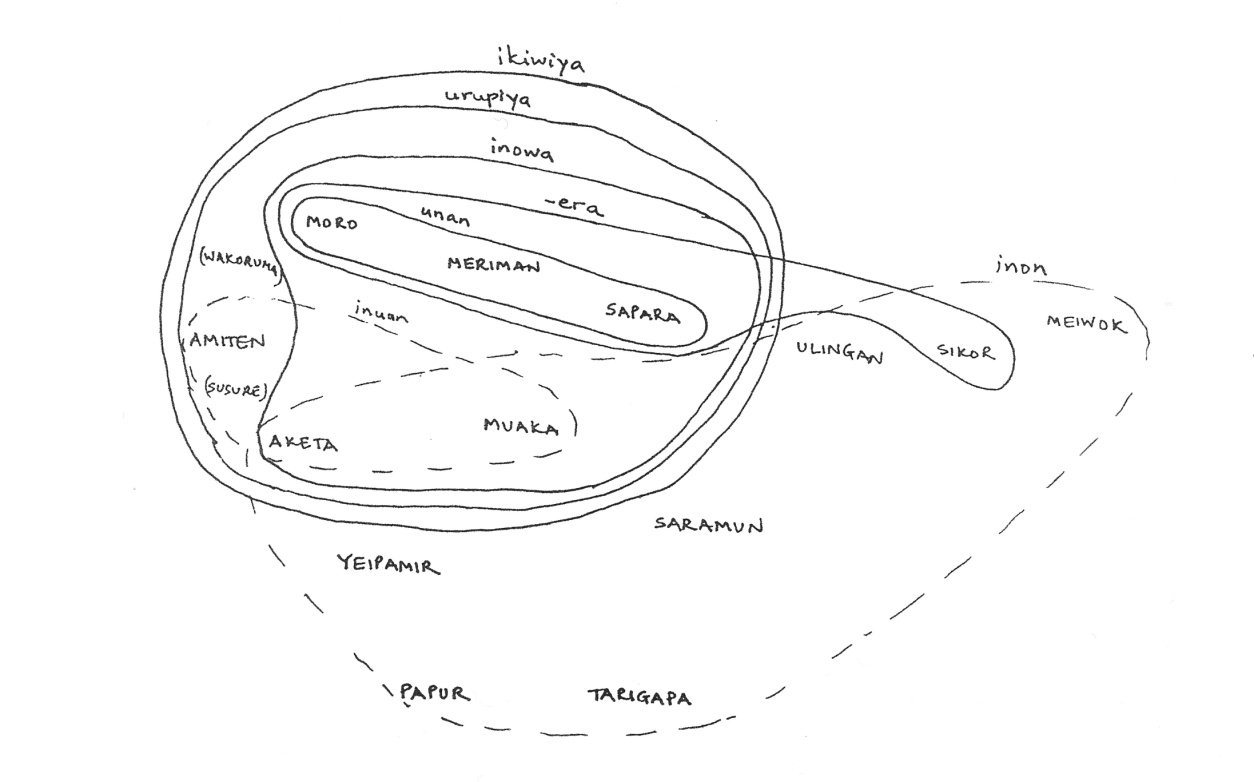
\includegraphics[width=\textwidth]{figures/1-distribution_of_some_pronounciation_differnces_map.jpeg}
\end{figure}

What complicates the dialect division is the fact that sometimes the same pronunciation, deviant from the more common way of pronouncing a word, can be found in villages far apart like Aketa and Meiwok: (\textstyleStyleVernacularWordsItalic{imakuna} rather than \textstyleStyleVernacularWordsItalic{umakuna} `neck'), or Papur,  Moro and Mereman villages and the Ulingan group (\textstyleStyleVernacularWordsItalic{epia} rather than \textstyleStyleVernacularWordsItalic{ipia} `rain'). Also, there is no clear pattern of pronunciation differences between villages; sometimes the differences are opposite in the case of two vocabulary items. The word for `many' in the Muaka dialect\footnote{Excluding Amiten/Susure/Wakoruma} is \textstyleStyleVernacularWordsItalic{inowa}, but the others pronounce it \textstyleStyleVernacularWordsItalic{unowa}, whereas the word for `ascend/go up' in the Muaka dialect is \textstyleStyleVernacularWordsItalic{urupiya}\emphs but in the other dialects it is \textstyleStyleVernacularWordsItalic{iripiya}. Likewise, the Ulingan group differs from the rest in the pronunciation of \textstyleStyleVernacularWordsItalic{omaiwia} `tongue' (vs. \textstyleStyleVernacularWordsItalic{omaiwa} in others) and \textstyleStyleVernacularWordsItalic{awulak} `sweet potato' (vs. \textstyleStyleVernacularWordsItalic{awuliak} in others), so the difference is almost exactly the reverse in the two cases.  

No grammatical differences have been found to exist between the dialects.  Neither are there social registers, nor special language for restricted uses like rituals. 

